\documentclass[mathserif]{beamer}

\usepackage{listings}
\usepackage{showexpl}
\usepackage{xfrac}
\usepackage{amsmath}
\usepackage{amsfonts}
\usepackage[T1]{fontenc}

%\usepackage{handoutwithnotes}

%\pgfpagesuselayout{3 on 1 with notes}[a4paper,border shrink=5mm]

%\pgfpageslogicalpageoptions{1}{border code=\pgfusepath{stroke}}
%\pgfpageslogicalpageoptions{2}{border code=\pgfusepath{stroke}}
%\pgfpageslogicalpageoptions{3}{border code=\pgfusepath{stroke}}


\lstdefinestyle{latexsty}{
	language={[LaTeX]TeX},
    basicstyle=\small\ttfamily,
    breaklines=true,
    breakindent=0pt, 
    backgroundcolor=\color{lightgray},
    numbers=none, numberstyle=\tiny, stepnumber=1, numbersep=5pt,
    commentstyle=\color{red},
    showstringspaces=false,
    keywordstyle=\color{blue}\bfseries,
    morekeywords={align,begin},
    tabsize=2,
    pos=b
}

\usetheme{default}
\useoutertheme{infolines}
\usecolortheme[RGB={166,5,20}]{structure}
%\setbeamertemplate{items}[circle]
\setbeamertemplate{blocks}[rounded][shadow=false]
\setbeamertemplate{navigation symbols}{}
\setbeamercovered{transparent}

\title{\LaTeX: An Introduction (Part 2)}
\subtitle{University Graduate College Training Course}
\author[Martin Chorley]{Dr Martin Chorley}
\institute[COMSC]{School of Computer Science \& Informatics, Cardiff University}
\date[21/02/13]{February 21st, 2014}


\begin{document}

%--------------- slide -------------------
\begin{frame}{Presentations in \LaTeX}

\vfill
\LaTeX\ is not limited to producing scientific papers, reports, articles or theses. It can also be used for many other types of documents, including presentations.
\vfill
In fact, all the presentations and handouts used in this course have been written in \LaTeX. 
\vfill
\end{frame}

%--------------- slide -------------------
\begin{frame}[fragile]
\frametitle{The \texttt{beamer} Document Class}

\vfill
To create presentations in \LaTeX, we use the \texttt{beamer} document class. It makes creating presentations relatively simple, but is sufficiently advanced to be able to manage quite complex tasks if we  desire.
\vfill
A simple example:
\vfill
\begin{lstlisting}[style=latexsty]
\documentclass{beamer}
\usetheme{default}
\begin{document}

    \begin{frame}
        \frametitle{A Slide}
        Hello World!
    \end{frame}

\end{document}
\end{lstlisting}
\vfill
\end{frame}

%--------------- slide -------------------
\frame{
\frametitle{A Simple Example}

\vfill
The sample code on the previous slide results in the presentation slide below:
\vfill
\begin{center}
	\fbox{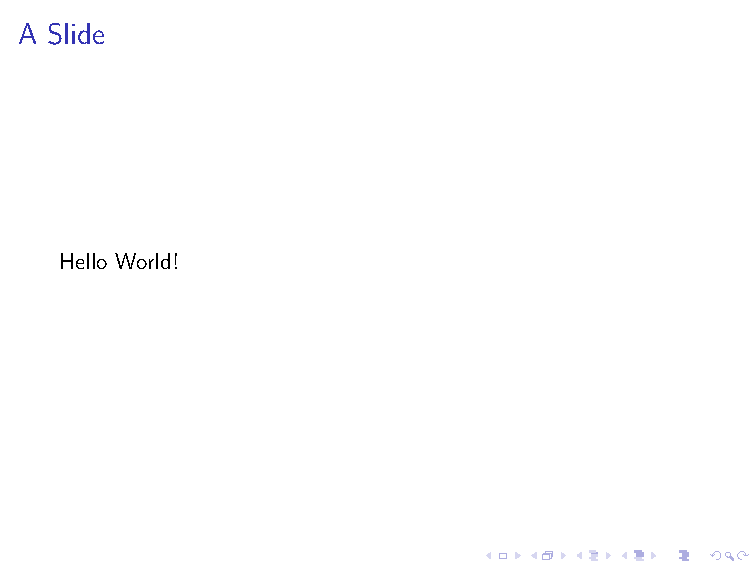
\includegraphics[width=0.6\textwidth]{example1.pdf}}
\end{center}
\vfill
}

%--------------- slide -------------------
\begin{frame}[fragile]
\frametitle{Frames \& Slides}

\vfill
What we normally call `slides' in presentations, \texttt{beamer} refers to as \texttt{frames}. The \texttt{frame} environment is used to define each slide in our presentation; the content for our slides is written within this environment.
\vfill
\begin{lstlisting}[style=latexsty]
    \begin{frame}
        \frametitle{A Slide}
        Hello World!
    \end{frame}

\end{lstlisting}
\vfill
We can include as many slides as we desire by repeating the \texttt{frame} environment for each slide.
\vfill
\end{frame}

%--------------- slide -------------------
\begin{frame}[fragile]
\frametitle{Frame Shortand}

\vfill
Rather than typing \texttt{{\textbackslash}begin\{frame\} \ldots {\textbackslash}begin\{frame\}} for each slide, we can use the shortcut \texttt{{\textbackslash}frame\{ \ldots \}}
\vfill
So:
\vfill
\begin{lstlisting}[style=latexsty]
    \begin{frame}
        \frametitle{A Slide}
        Hello World!
    \end{frame}
\end{lstlisting}
\vfill
and:
\vfill
\begin{lstlisting}[style=latexsty]
    \frame{
        \frametitle{A Slide}
        Hello World!
    }
\end{lstlisting}
\vfill
are the same thing.
\vfill
\end{frame}

%--------------- slide -------------------
\begin{frame}[fragile]
\frametitle{Frame Titles}

\vfill
\texttt{beamer} allows us to specify the title of a slide in two different ways:
\vfill
\begin{enumerate}
	\item Using the \texttt{{\textbackslash}frametitle} command as in our previous example
	\item By specifying the title as an argument on the frame environment:
\end{enumerate}
\vfill
\begin{lstlisting}[style=latexsty]
    \begin{frame}{A Slide}
        Hello World!
    \end{frame}
\end{lstlisting}
\vfill
Either way is fine. The first method is the older method and the second is only supported in newer versions of beamer. If you are using \texttt{{\textbackslash}frame\{ \ldots \}} you will need to use the first method.

\end{frame}

%--------------- slide -------------------
\begin{frame}[fragile]
\frametitle{Metadata}

\vfill
We specify author, title and date information in the preamble of the document.
\vfill
\begin{lstlisting}[style=latexsty]
	\title[optional short title]{Title of Presentation}
	\subtitle{An optional extra subtitle}
	\author[optional short author name]{Author name}
	\institute[optional short name]{Institute name}
	\date[short date]{Date information}
\end{lstlisting}
\vfill
The optional short version of the title, author and date information is included for display on slide footers etc.
\vfill
\end{frame}

%--------------- slide -------------------
\begin{frame}[fragile]
\frametitle{Title Page}

\vfill
Once we have specified the document metadata, we can use the \texttt{{\textbackslash}titlepage} command to insert a title page into our presentation
\vfill
\begin{lstlisting}[style=latexsty]
    \title[\LaTeX]{\LaTeX\ for Beginners}
    \subtitle{University Graduate College Training Course}
    \author[MJC]{Martin Chorley}
    \institute[COMSC]{School of Computer Science \& Informatics \\ Cardiff University}
    \date[Feb 2013]{February 1st 2013}

    \begin{frame}{}
        \titlepage
    \end{frame}
\end{lstlisting}
\vfill
\end{frame}

%--------------- slide -------------------
\frame{
\frametitle{Title Page Example}

\vfill
The sample code on the previous slide results in the presentation slide below:
\vfill
\begin{center}
	\fbox{
\includegraphics[width=0.6\textwidth]{example2.pdf}}
\end{center}
\vfill
}

%--------------- slide -------------------
\begin{frame}[fragile]
\frametitle{Themes}

\vfill
\texttt{beamer} allows us to change the appearance of our slides by using themes.
\vfill
\begin{lstlisting}[style=latexsty]
	\documentclass{beamer}
	\usetheme{default}
\end{lstlisting}
\vfill
Some of the available themes are:
\vfill
\begin{center}
	\begin{tabular}{l | l | l | l | l}
Antibes & Boadilla & Berkeley & Berlin & Copenhagen \\
Darmstadt & Dresden & Frankfurt & Goettingen & Hannover \\
Ilmenau & JuanLesPins & Luebeck & Madrid & Malmoe \\
Marburg & Montpellier & PaloAlto & Pittsburgh & Rochester \\
Singapore & Szeged & Warsaw & boxes & default \\
	\end{tabular}
\end{center}
\vfill
\end{frame}

%--------------- slide -------------------
\frame{
\frametitle{\texttt{default} Theme}

\vfill
\begin{center}
	\fbox{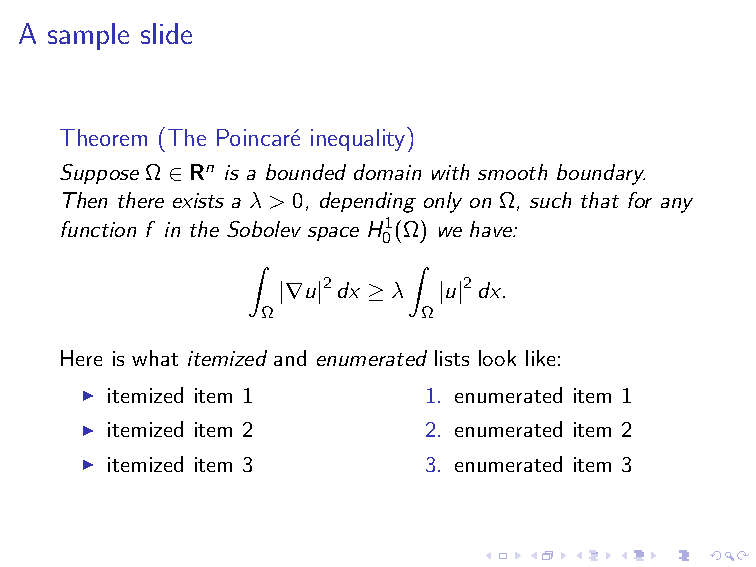
\includegraphics[width=0.8\textwidth]{example3.pdf}}
\end{center}
\vfill
}

%--------------- slide -------------------
\frame{
\frametitle{\texttt{Berkeley} Theme}

\vfill
\begin{center}
	\fbox{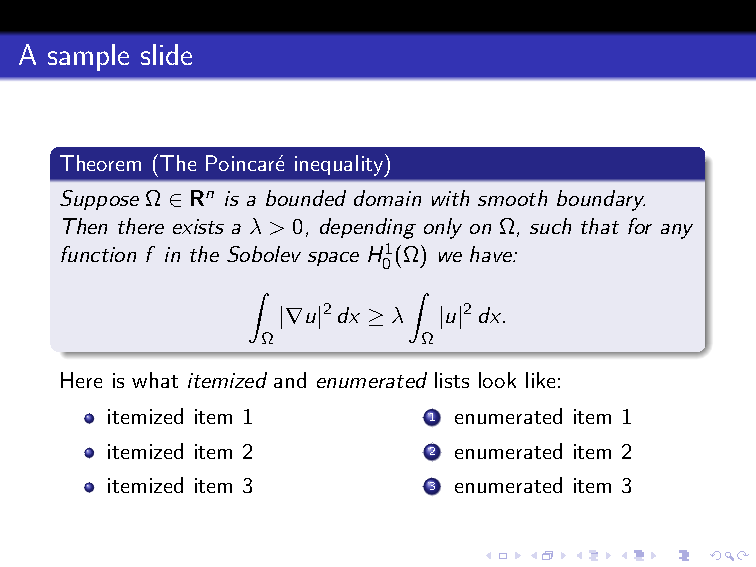
\includegraphics[width=0.8\textwidth]{example4.pdf}}
\end{center}
\vfill
}

%--------------- slide -------------------
\frame{
\frametitle{\texttt{Boadilla} Theme}

\vfill
\begin{center}
	\fbox{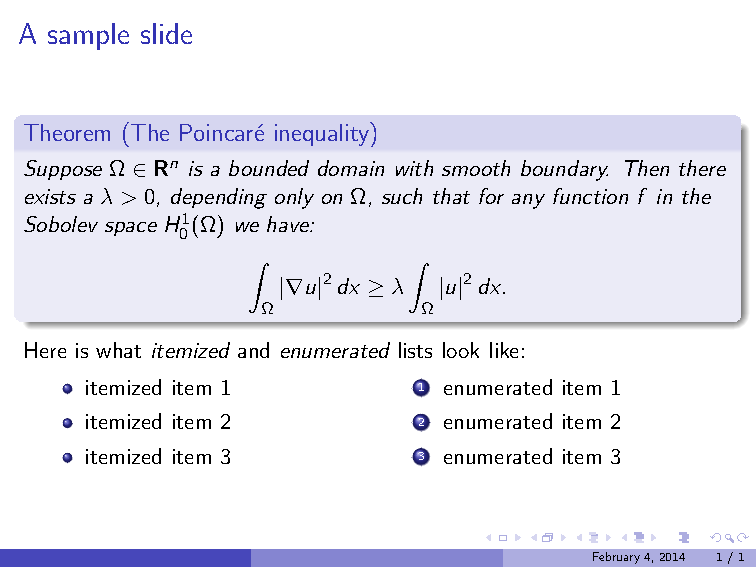
\includegraphics[width=0.8\textwidth]{example5.pdf}}
\end{center}
\vfill
}

%--------------- slide -------------------
\begin{frame}[fragile]
\frametitle{Customising Themes}

\vfill
We can customise \texttt{beamer} themes in many ways. 
\vfill
Changing the \texttt{outertheme} with the \texttt{{\textbackslash}useoutertheme\{\ldots\}} command will change the header and footer of each slide. Available outer themes include:
\vfill
\begin{center}
	\begin{tabular}{l | l | l | l}
infolines & miniframes & shadow & sidebar \\
smoothbars & smoothtree & split & tree \\
	\end{tabular}
\end{center}
\vfill
Changing the \texttt{innertheme} with the \texttt{{\textbackslash}useinnertheme\{\ldots\}} command will change the inner elements (bullets, boxes) of each slide. Available inner themes include:
\vfill
\begin{center}
	\begin{tabular}{l | l | l | l}
rectangles & circles & inmargin & rounded
	\end{tabular}
\end{center}
\vfill

\end{frame}

%--------------- slide -------------------
\begin{frame}[fragile]
\frametitle{Customising Themes}
\vfill
We can set the colour of elements on slides individually:
\vfill
\begin{lstlisting}[style=latexsty]
	\setbeamercolor{frametitle}{fg=red}
\end{lstlisting}
\vfill
Similarly, we can change the font of particular elements:
\vfill
\begin{lstlisting}[style=latexsty]
	\setbeamerfont{title}{family=\rm}
\end{lstlisting}
\vfill
Alternatively we can customise the colour and fonts of \texttt{beamer} themes using the \texttt{{\textbackslash}usefonttheme\{\ldots\}} command and the \texttt{{\textbackslash}usecolortheme\{\ldots\}} command.
\vfill
\end{frame}

%--------------- slide -------------------
\begin{frame}[fragile]
\frametitle{Customising Themes - Colour}
\vfill
Recall the \texttt{Boadilla} theme?:
\vfill
\begin{center}
	\fbox{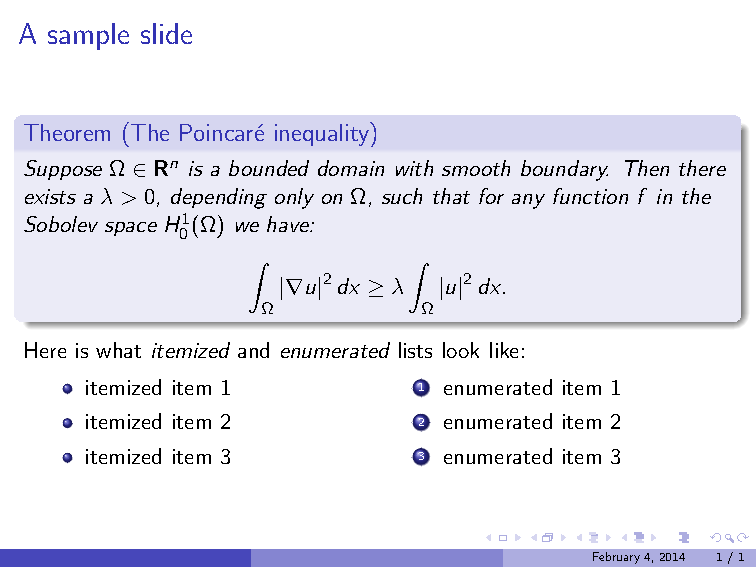
\includegraphics[width=0.5\textwidth]{example5.pdf}}
\end{center}
\vfill
The slide element structure is based around the colour blue. We can change this with the \texttt{{\textbackslash}usecolortheme\{\ldots\}} command
\end{frame}

%--------------- slide -------------------
\begin{frame}[fragile]
\frametitle{Customising Themes - Colour}
\vfill
If we change the theme to red:
\vfill
\begin{lstlisting}[style=latexsty]
	\usecolortheme[named=green]{structure}
\end{lstlisting}
\vfill
The structure elements of the slide change to the colour specified:
\vfill
\begin{center}
	\fbox{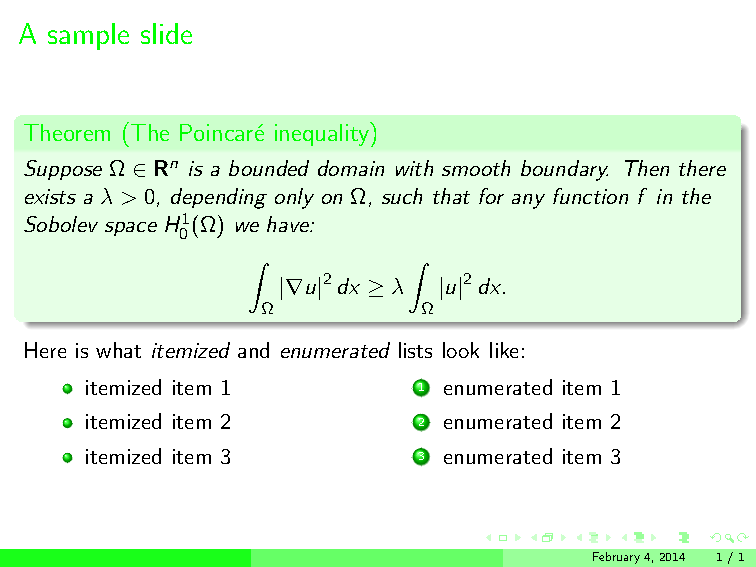
\includegraphics[width=0.5\textwidth]{example6.pdf}}
\end{center}
\vfill
\end{frame}

%--------------- slide -------------------
\begin{frame}[fragile]
\frametitle{Customising Themes - Colour}
\vfill
We can even specify our own colours. So, to match the Cardiff University official colour:
\vfill
\begin{lstlisting}[style=latexsty]
	\usecolortheme[RGB={166,5,20}]{structure}
\end{lstlisting}
\vfill
\begin{center}
	\fbox{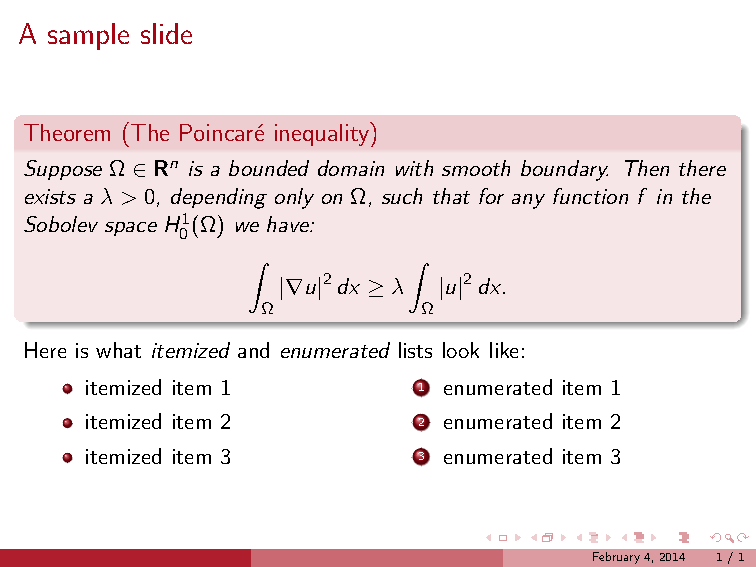
\includegraphics[width=0.5\textwidth]{example7.pdf}}
\end{center}
\vfill
\end{frame}

%--------------- slide -------------------
\begin{frame}[fragile]
\frametitle{Customising Slides - Removing Navigation}
\vfill
\texttt{beamer} includes navigation items on slide output for moving through the presentation. These are usually unnecessary and can be removed:
\vfill
\begin{lstlisting}[style=latexsty]
	\setbeamertemplate{navigation symbols}{} 
\end{lstlisting}
\vfill
\begin{center}
	\fbox{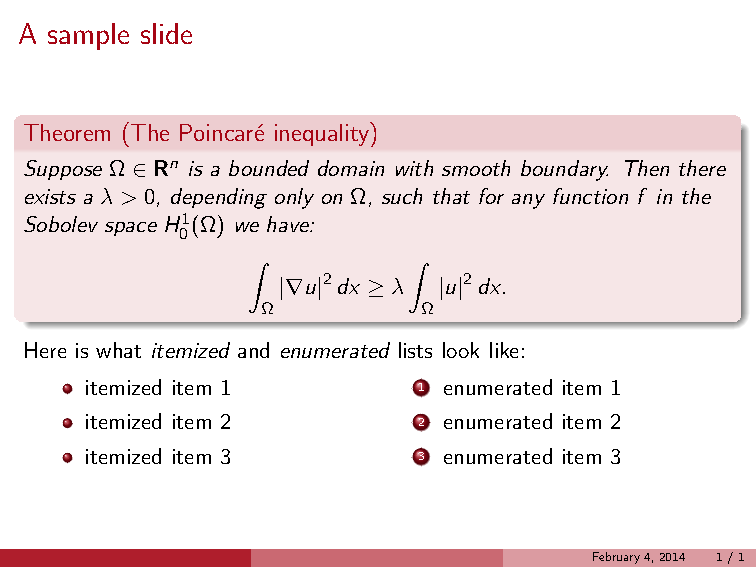
\includegraphics[width=0.5\textwidth]{example8.pdf}}
\end{center}
\vfill
\end{frame}

%--------------- slide -------------------
\begin{frame}[fragile]
\frametitle{Customising Slides - Adding a footer}
\vfill
Some themes come with a footer already included, some do not. Using the \texttt{{\textbackslash}useoutertheme\{infolines\}} command will add a footer to any theme that does not have one.
\vfill
\begin{lstlisting}[style=latexsty]
	\documentclass{beamer} 
	\usecolortheme[named=red]{structure} 
	\useoutertheme{infolines} 
	\usetheme{Rochester} 
\end{lstlisting}
\vfill
This command must come \emph{before} the command to set the theme.
\vfill
\end{frame}


%--------------- slide -------------------
\begin{frame}[fragile]
\frametitle{Removing Decoration}
\vfill
If you have a lot of information or a large picture to display on a slide and want to remove the decoration, add the \texttt{[plain]} option to the frame environment:
\vfill
\begin{lstlisting}[style=latexsty]
\begin{frame}[plain] 
...
\end{lstlisting}
\vfill
\begin{center}
	\fbox{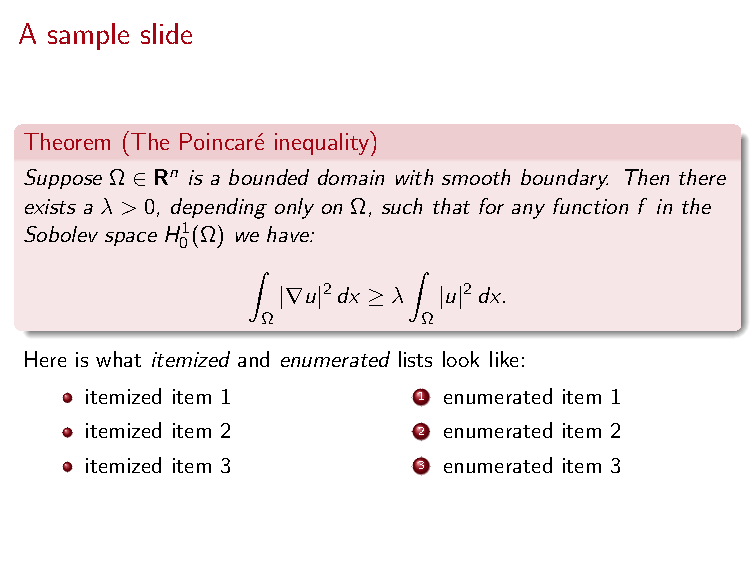
\includegraphics[width=0.5\textwidth]{example9.pdf}}
\end{center}
\vfill
\end{frame}


%--------------- slide -------------------
\begin{frame}[fragile]
\frametitle{Columns}
\vfill
It is possible to split slides into columns
\vfill
\begin{lstlisting}[style=latexsty]
	\begin{frame}{Columns}
	    Here's a line that goes all the way across the slide, it will be followed by two columns
	    \begin{columns}
	        \begin{column}{0.3\textwidth}
	            Here's a column that takes up 30 percent of the width of the slide
	        \end{column}
	        \begin{column}{0.5\textwidth}
	            Here's a column that takes up 50 percent of the width of the slide
	        \end{column}
	    \end{columns}
	    Finally here's a line that goes all the way across the slide again.
\end{lstlisting}
\vfill
\end{frame}

%--------------- slide -------------------
\begin{frame}[fragile]
\frametitle{Columns Example}
\vfill
\begin{center}
	\fbox{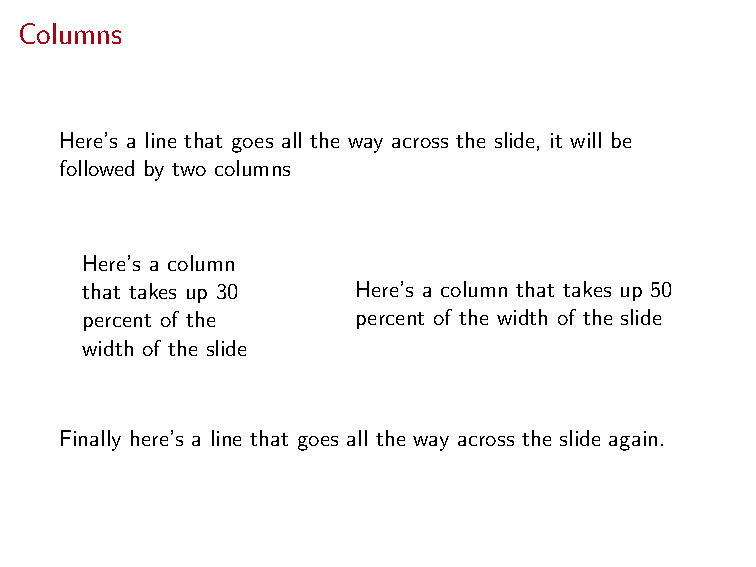
\includegraphics[width=0.8\textwidth]{example10.pdf}}
\end{center}
\vfill
\end{frame}

%--------------- slide -------------------
\begin{frame}[fragile]
\frametitle{Blocks}
\vfill
It is possible to put text in blocks within slides, these can be titled or optionally can have a blank title
\vfill
\begin{lstlisting}[style=latexsty]
\begin{frame}{Blocks}
	\begin{block}{A Block}
	    Here's a block of text in a marked block with a title
	\end{block}
	\begin{block}{}
	    Here's a block of text in a marked block with an empty title
	\end{block}
	\begin{alertblock}{an Alert block}
	    This is a block of text in an alert block
	\end{alertblock}
	\begin{exampleblock}{an Example block}
	    This is a block of text in an example block
	\end{exampleblock}
\end{lstlisting}
\vfill
\end{frame}

%--------------- slide -------------------
\begin{frame}[fragile]
\frametitle{Blocks Example}
\vfill
\begin{center}
	\fbox{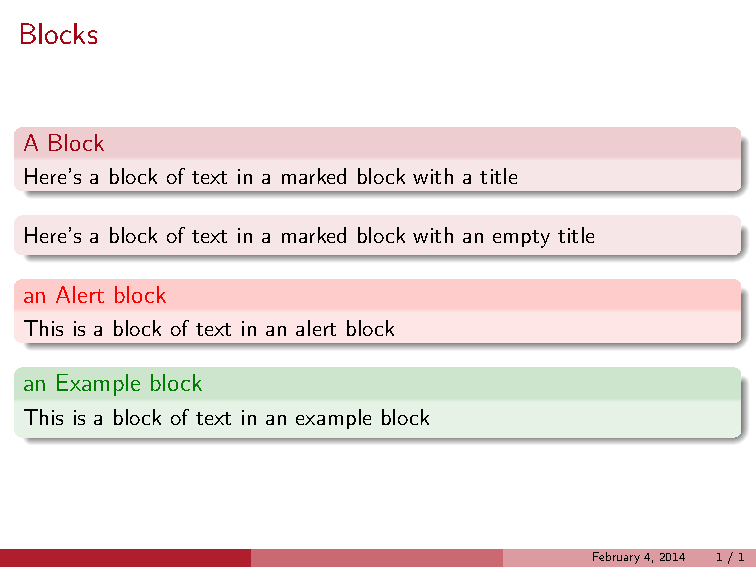
\includegraphics[width=0.8\textwidth]{example11.pdf}}
\end{center}
\vfill
\end{frame}

%--------------- slide -------------------
\begin{frame}[fragile]
\frametitle{Animation}
\vfill
\texttt{beamer} is capable of adding animation to slides. The \texttt{{\textbackslash}pause} command causes \texttt{beamer} to output slides at different stages of construction, so that items appear as we advance through the slides.
\vfill
\begin{lstlisting}[style=latexsty]
\begin{frame}[plain]
This sentence will appear first \\
\pause
Then this sentence \\
\pause
Finally this sentence \\
\end{lstlisting}
\vfill
\end{frame}

%--------------- slide -------------------
\begin{frame}
This sentence will appear first \\
\pause
Then this sentence \\
\pause
Finally this sentence \\
\end{frame}

%--------------- slide -------------------
\begin{frame}[fragile]
\frametitle{Animation}
\vfill
A shorthand for pause when using the \texttt{{\textbackslash}itemize} environment is to use\texttt{{\textbackslash}itemize}[\textless +-\textgreater]. This effectively acts as a \texttt{{\textbackslash}pause} command before each item in the list:
\vfill
\begin{lstlisting}[style=latexsty]
\begin{itemize}[<+->]
	\item The first item
	\item The second item
	\item The third item
\end{itemize}
\end{lstlisting}
\vfill
\end{frame}

%--------------- slide -------------------
\begin{frame}
\begin{itemize}[<+->]
	\item The first item
	\item The second item
	\item The third item
\end{itemize}
\end{frame}

%--------------- slide -------------------
\begin{frame}[fragile]
\frametitle{Complex Animation}
\vfill
A fine grained control of the order and duration of items being visible can be had with many environments and commands by specifying on which slides an item should appear.
\vfill
\begin{lstlisting}[style=latexsty]
\begin{itemize}
	\item<1-> This item will appear from the first slide onwards
	\item<2-> This item will appear from the second slide onwards
	\item<3-> This item will appear from the third slide onwards
	\item<2-3> This item will appear on the second slide until the third
	\item<4-> This item will appear on the fourth slide
\end{itemize}
\end{lstlisting}
\vfill
\end{frame}

%--------------- slide -------------------
\begin{frame}
\begin{itemize}
	\item<1-> This item will appear from the first slide onwards
	\item<2-> This item will appear from the second slide onwards
	\item<3-> This item will appear from the third slide onwards
	\item<2-3> This item will appear on the second slide until the third
	\item<4-> This item will appear on the fourth slide
\end{itemize}
\end{frame}


%--------------- slide -------------------
\begin{frame}[fragile]
\frametitle{Animation}
\vfill
There are also commands for controlling on which slides text appears: the \texttt{{\textbackslash}only\textless n-m\textgreater} command and \texttt{{\textbackslash}uncover\textless n-m\textgreater} commands.
\vfill
The \texttt{{\textbackslash}only\textless n-m\textgreater} command will only insert text on the specified slides.
\vfill
The \texttt{{\textbackslash}uncover\textless n-m\textgreater} command will insert text on all slides, but only `uncover' it on the specified slides. The rest of the time it will be covered according to the setting of \texttt{{\textbackslash}setbeamercovered}.
\vfill
\end{frame}

%--------------- slide -------------------
\begin{frame}[fragile]
\frametitle{\texttt{{\textbackslash}uncover}}
\vfill
The \texttt{{\textbackslash}uncover\textless n-m\textgreater} command will insert text on all slides, but only `uncover' it on the specified slides. The rest of the time it will be covered according to the setting of \texttt{{\textbackslash}setbeamercovered} (which could be \texttt{transparent} for example).
\vfill
\begin{lstlisting}[style=latexsty]
\uncover<1->{This text is visible from slide 1 onwards \\}
\uncover<2-3>{This text is visible from slide 2 to slide 3 \\}
\uncover<3>{This text is visible on slide 3 \\} 
\uncover<4->{This text is visible from slide 4 onwards}
\end{lstlisting}
\vfill
\end{frame}

%--------------- slide -------------------
\begin{frame}
\uncover<1->{This text is visible from slide 1 onwards \\}
\uncover<2-3>{This text is visible from slide 2 to slide 3 \\}
\uncover<3>{This text is visible on slide 3 \\}
\uncover<4->{This text is visible from slide 4 onwards}
\end{frame}

%--------------- slide -------------------
\begin{frame}[fragile]
\frametitle{\texttt{{\textbackslash}only}}
\vfill
The \texttt{{\textbackslash}only\textless n-m\textgreater} command will only insert text on the specified slides. At all other times, the text will not be rendered.
\vfill
\begin{lstlisting}[style=latexsty]
\only<1->{This text is visible from slide 1 onwards \\} 
\only<2-3>{This text is visible from slide 2 to slide 3 \\}
\only<3>{This text is visible on slide 3 \\} 
\only<4->{This text is visible from slide 4 onwards}
\end{lstlisting}
\vfill
\end{frame}

%--------------- slide -------------------
\begin{frame}[fragile]
\only<1->{This text is visible from slide 1 onwards \\}
\only<2-3>{This text is visible from slide 2 to slide 3 \\} 
\only<3>{This text is visible on slide 3 \\} 
\only<4->{This text is visible from slide 4 onwards}
\end{frame}

%--------------- slide -------------------
\begin{frame}[fragile]
\frametitle{Handouts}
\vfill
We have seen that \texttt{beamer} creates animation by creating duplicate slides with intermediate steps displayed.
\vfill
These intermediate slides are not necessary when creating handouts to give to the audience.
\vfill
Setting \texttt{beamer} to `handout' mode will suppress this extra slide creation, and create slides with all steps of the animation on them.
\vfill
\begin{lstlisting}[style=latexsty]
\documentclass[handout]{beamer}
\end{lstlisting}
\vfill

\end{frame}

%--------------- slide -------------------
\begin{frame}
\frametitle{Exercise 5}

\begin{center}
\vfill
Use the \texttt{beamer} document class to create a presentation
\vfill
\end{center}
\end{frame}

\end{document}